\documentclass[spanish, 10pt,a4paper]{article}
\usepackage[spanish]{babel}
\usepackage[utf8]{inputenc}
\usepackage{textcomp}
\usepackage{hyperref}
\usepackage[pdftex]{graphicx}
\usepackage{epsfig}
\usepackage{amsmath}
\usepackage{hyperref}
\usepackage{amssymb}
\usepackage{color}
\usepackage{graphics}
\usepackage{amsthm}
\usepackage{subcaption}
\usepackage{caratula}
\usepackage{fancyhdr,lastpage}
\usepackage[paper=a4paper, left=1.4cm, right=1.4cm, bottom=1.4cm, top=1.4cm]{geometry}
\usepackage[table]{xcolor} % color en las matrices
\usepackage[font=small,labelfont=bf]{caption} % caption de las figuras en letra mas chica que el texto
\usepackage{listings}
\usepackage{float}
\usepackage{pdfpages}
\usepackage{amsfonts}


\color{black}

%%%PAGE LAYOUT%%%
\topmargin = -1.2cm
\voffset = 0cm
\hoffset = 0em
\textwidth = 48em
\textheight = 164 ex
\oddsidemargin = 0.5 em
\parindent = 2 em
\parskip = 3 pt
\footskip = 7ex
\headheight = 20pt
\pagestyle{fancy}
\lhead{IS1 - Trabajo Pr\'actico 1} % cambia la parte izquierda del encabezado
\renewcommand{\sectionmark}[1]{\markboth{#1}{}} % cambia la parte derecha del encabezado
\rfoot{\thepage}
\cfoot{}
\numberwithin{equation}{section} %sets equation numbers <chapter>.<section>.<subsection>.<index>

\newcommand{\figurewidth}{1\textwidth}

\newcommand{\tuple}[1]{\ensuremath{\left \langle #1 \right \rangle }}
\newcommand{\Ode}[1]{\small{$\mathcal{O}(#1)$}}


%El siguiente paquete permite escribir la caratula facilmente
\hypersetup{
  pdftitle={ IS1 - TP1 },
  colorlinks,
  citecolor=black,
  filecolor=black,
  linkcolor=black,
  urlcolor=black 
}

\materia{Ingeniería de Software I}

\titulo{Trabajo Práctico 1}

\subtitulo{Informe y diagramas.}

\grupo{Grupo 2}

\integrante{De Sousa Bispo, Germán}{359/12}{germandesousa@gmail.com}
\integrante{Fernandez, Esteban}{691/12}{esteban.pmf@gmail.com}
\integrante{Kodelia, Erika Natasha}{767/11}{erikankodelia@gmail.com}
\integrante{Mongi Badia, Martín}{422/13}{martinmongi@gmail.com}
\integrante{Sánchez Cano, Gonzalo}{}{xeneize__86@hotmail.com}
\integrante{Wright, Carolina}{876/12}{wright.carolina@gmail.com}

 
\begin{document}
{ \oddsidemargin = 2em
	\headheight = -20pt
	\maketitle
}
	\tableofcontents
	\newpage

\section{Introducción}

	Para este Trabajo Práctico, se nos pidió especificar un sistema para reemplazar el Sistema Electoral Nacional actual. El objetivo de este nuevo sistema es volverlo más moderno, ágil y transparente. Dado que el formato de la votación no presenta cambios, el sistema debe proveer las mismas modalidades de voto que el sistema actual; es decir, el sistema debe permitir el voto de una lista completa, el voto por categoría (o `corte de boleta') y el voto en blanco.
	
	Para este objetivo, se nos pide diseñar el comportamiento de una máquina emisora de sufragios, a razón de una por cada mesa de votación, la que permita a los Electores efectuar el sufragio de una forma clara, transparente y secreta.
	
	A su vez, nuestro Sistema debe especificar el comportamiento del Centro de Cómputos Nacional, encargado de recibir los resultados desde todas las máquinas y procesar estos resultados, dando a conocer los resultados mientras las mesas se escrutan.
	
	En particular, nuestro sistema debe implementar las siguientes funcionalidades:
\begin{itemize}
\item Poder cargar y consultar el padrón electoral.
\item Poder cargar y consultar los candidatos disponibles para cada cargo.
\item Poder asignar al Presidente de Mesa para cada una de las mesas.
\item Pasadas las 18 horas, poder registrar y consultar los Resultados parciales y totales.
\item Poder calcular los candidatos electos para los cargos ejecutivos y legistlativos.
\item Poder cargar en las máquinas los candidatos antes del día electoral.
\item El Presidente de Mesa debe poder abrir y cerrar la mesa en el día electoral.
\item Poder garantizar al Elector la posibilidad de efectuar su sufragio en forma secreta.
\item Poder dar asistencia al Elector para el uso de las máquinas de sufragio, incluso en el caso de votantes no videntes o parcialmente discapacitados.
\item Poder dar a los fiscales la posibilidad de controlar los comicios.
\end{itemize}

	También, debemos especificar de que forma nuestro sistema a especificar almacenará los sufragios de los Electores. Debemos decidir entre varias alternativas: boleta impresa, digital en un medio de almacenamiento a designar, etc.
	
	En este informe, utilizamos diferentes técnicas para especificar un Sistema Electoral Nacional, tales como diagramas de contexto, actividad y clases, máquinas de estados finitos.


\section{Presunciones}
	Dada la estructura del sistema que se propuso en el trabajo práctico anterior, donde existen máquinas de sufragio comunicadas con servidores locales (por escuela) que a su vez se engloban bajo el Centro Nacional de Cómputo, asumimos que no van a ocurrir problemas con la comunicación entre estos aparatos (falta de Internet, rotura de los cables de red e imposibilidad de utilización de Wi-Fi). 
\par Por otro lado, el sistema permitirá el voto de personas con movilidad reducida así como también de personas no videntes. En caso de sufrir alguna discapacidad que no se contempla, el elector está justificado a no votar o a realizarlo con ayuda de un tutor.
\par Dado que el sistema permite el voto de personas con movilidad reducida, asumimos que las escuelas poseen acceso a, por lo menos, la planta baja para personas en silla de ruedas. 

\section{Vistas}
	A continuación se visualizarán los diagramas realizados junto con la explicación necesaria para cada tipo:
\subsection{Diagrama de Contexto}
	Se agrega el diagrama de contexto entregado en el trabajo práctico anterior con las modificaciones necesarias para adptarse a los O-refinamientos elegidos. Esto corresponde a no realizar una autenticación por parte del Elector a la máquina de sufragio a la hora de realizar la votación (alcanza con insertar la boleta). Además, la habilitación del modo audio de la máquina de sufragio por parte del Presidente de Mesa se realiza solamente a través de la inserción de los auriculares. 
\par El diagrama de contexto resultante es el siguiente:

\vspace{\baselineskip}
    \begin{center}
                \includegraphics[scale=0.40]{imagenes/contexto/DiagramaDeContextoTP2.png}
                \\
                \vspace{1pt}
                \footnotesize\textit{}
        \end{center}
\vspace{\baselineskip}

\clearpage
\subsection{Diagrama de Caso de Uso}

\vspace{\baselineskip}
    \begin{center}
                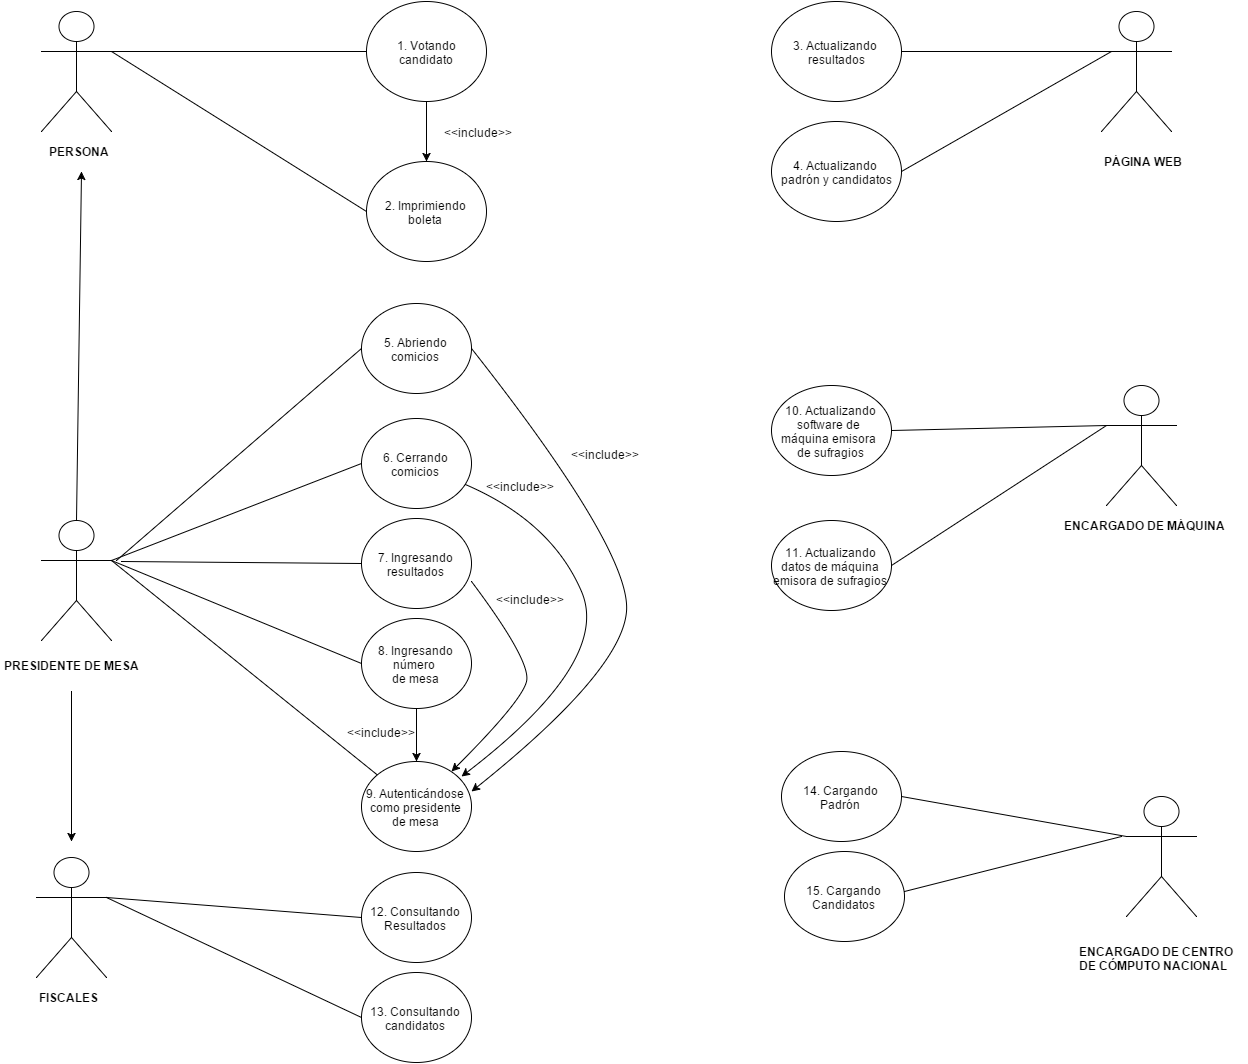
\includegraphics[scale=0.40]{imagenes/CasosDeUso.png}
                \\
                \vspace{1pt}
                \footnotesize\textit{}
        \end{center}
\vspace{\baselineskip}

\newpage

\noindent\textbf{Detalle de Casos de Uso:}\\

\noindent\textbf{Caso de Uso: 1. Votando candidatos}\\
\textbf{Actor: } Persona.\\
\textbf{Pre: } Se abrieron los comicios.\\
\textbf{Post: } La persona logra registrar su voto.\\
\begin{table}[H]
  \centering
\bgroup
\def\arraystretch{1.3}
  \begin{tabular}{p{9cm} | p{7cm}}
    \hline
    Curso Normal & Curso Alternativo \\
    \hline
    \hline    
    1. La \textbf{\textit{persona}} ingresa la \textit{boleta de votación}. 
    & \\
    
    \hline
    2. La \textbf{\textit{máquina de sufragio}} brinda toda la información en este CU, tanto por pantalla como por audio a través de una salida por auricular.
    &
    \\
    
    \hline
    3 La \textbf{\textit{máquina de sufragio}} verifica que sea una \textit{boleta de votación}.
    & 
    3.1 En el caso que no sea una boleta válida, la \textbf{\textit{máquina de sufragio}} entrega el mensaje de \textit{''Error de boleta''}
    \\
    
    \hline
    4 La \textbf{\textit{máquina de sufragio}} le brinda a la persona, las opciones de \textit{''votar lista completa''} y \textit{''votar por categorías''}.
    & 
    4.1 En el caso en que no se pueda mostrar la información necesaria, la \textbf{\textit{máquina de sufragio}} entrega el mensaje de \textit{''Error de interfaz''}
    \\
    
    \hline
    5 La \textbf{\textit{persona}} elige una de las dos opciones mostradas en el paso anterior.
    & \\
    
    \hline
    6 Si la \textbf{\textit{persona}} eligió lista completa, Ir al \textbf{\textit{paso 15}}.
    & \\
    
    \hline
    7 La \textbf{\textit{máquina de sufragio}} muestra como opciones distintas a cada uno de los candidatos de una categoría y otra opción de \textit{''votar en blanco''}.
    & 
    7.1 En el caso en que no se pueda mostrar la información necesaria, la \textbf{\textit{máquina de sufragio}} entrega el mensaje de \textit{''Error de interfaz''}
    \\
    
    \hline
    8 La \textbf{\textit{persona}} elige una de las opciones mostradas en el paso anterior.
    & \\
    
    \hline
    9 La \textbf{\textit{máquina de sufragio}} verifica que se hayan votado todas las categorías. Si falta votar alguna categoría, continúo con la siguiente categoría, ir al \textbf{\textit{paso 7}}.
    & \\
    
    \hline
    10 La \textbf{\textit{máquina de sufragio}} mostrará la elección de cada uno de los candidatos elegidos por la persona, junto con un botón de aceptar y otro de cancelar para que la misma pueda verificarlos.
    & \\
    
    \hline
    11 La \textbf{\textit{persona}} confirmará que desea realizar esa votación.
     En el caso en que la \textbf{\textit{persona}} no desee confirmar la votación y haya elegido realizarla nuevamente, ir al \textbf{\textit{paso 3}}.\\
    
    \hline
    12 La \textbf{\textit{máquina de sufragio}} registra el voto.
    & 
    12.1 En el caso en que no se pueda registrar el voto, la \textbf{\textit{máquina de sufragio}} entrega el mensaje de \textit{''Error de registración''}
    \\
    
    \hline
    13 La \textbf{\textit{máquina de sufragio}} imprime la boleta con la selección de candidatos incluyendo el caso de uso \textbf{2. Imprimiendo boleta}.
    & 
    \\
    
    \hline
    14 Ir al  \textbf{\textit{paso 17}}
    & \\
    
    \hline
    15 La \textbf{\textit{máquina de sufragio}} muestra como opciones distintas a cada uno de las listas completas de los candidatos y otra opción de \textit{''votar en blanco''}.
    & 
    15.1 En el caso en que no se pueda mostrar la información necesaria, la \textbf{\textit{máquina de sufragio}} entrega el mensaje de \textit{''Error de interfaz''}
    \\
    
    \hline
    16 La \textbf{\textit{persona}} elige una de las opciones mostradas en el paso anterior. Ir al \textbf{\textit{paso 10}}.
    & \\
    \hline

    \hline
    17 Fin de Caso de Uso.
    & \\
  \end{tabular}
\egroup
\end{table}


\newpage
\noindent\textbf{Caso de Uso: 2. Imprimiendo boleta}\\
\textbf{Actor: } Persona.\\
\textbf{Pre: } Se confirmó el voto y se encuentra ingresada la boleta de votación.\\
\textbf{Post: } Se imprime la boleta.\\
\begin{table}[H]
  \centering
\bgroup
\def\arraystretch{1.3}
  \begin{tabular}{p{9cm} | p{7cm}}
    \hline
    Curso Normal & Curso Alternativo \\
    \hline
    \hline    
    1. La \textbf{\textit{persona}} selecciona la opción de \textit{''Imprimir boleta''}. 
    & \\
    
    \hline
    2. La \textbf{\textit{máquina de sufragio}} imprime en la boleta los candidatos elegidos por la \textbf{\textit{persona}} y devuelve la boleta.
    &
    2.1 En el caso en que no se pueda imprimir la boleta, la \textbf{\textit{máquina de sufragio}} entrega el mensaje de \textit{''Error de impresión''}
    \\
    
    \hline
    3 Fin de CU
    & \\
    \hline
  \end{tabular}
\egroup
\end{table}


\noindent\textbf{Caso de Uso: 3. Actualizando resultados}\\
\textbf{Actor: } Página web.\\
\textbf{Pre: } Se cerraron los comicios.\\
\textbf{Post: } Se actualiza la información de los resultados en la página web.\\
\begin{table}[H]
  \centering
  \begin{tabular}{p{9cm} | p{7cm}}
    \hline
    Curso Normal & Curso Alternativo \\
    \hline
    \hline    
    1. La \textbf{\textit{Página web}} consulta resultados al \textbf{\textit{Centro de Cómputo Nacional}}. 
    & \\
    
    \hline
    2. El \textbf{\textit{Centro de Cómputo Nacional}} brinda satisfactoriamente la información a la página web
    & 
    2.1 Si el \textbf{\textit{Centro de Cómputo Nacional}} no puede brindar la información, se mostrará un mensaje de \textit{''Error de actualización de resultados''} en la página web.
    \\
    
    \hline
    3. La \textbf{\textit{Página web}} actualizará los resultados en la página web.
    & \\
    \hline
  \end{tabular}
\end{table}


\noindent\textbf{Caso de Uso: 4. Actualizando padrón y candidatos}\\
\textbf{Actor: } Página web.\\
\textbf{Pre: } Faltan por lo menos 24hs para la apertura de los comicios.\\
\textbf{Post: } Se actualiza la información del padrón y de los candidatos en la página web.\\
\begin{table}[H]
  \centering
  \begin{tabular}{p{9cm} | p{7cm}}
    \hline
    Curso Normal & Curso Alternativo \\
    \hline
    \hline    
    1. La \textbf{\textit{Página web}} consulta el padrón y los candidatos al \textbf{\textit{Centro de Cómputo Nacional}}. 
    & \\
    
    \hline
    2. El \textbf{\textit{Centro de Cómputo Nacional}} brinda satisfactoriamente la información a la \textbf{\textit{Página web}}
    & 
    2.1 Si el \textbf{\textit{Centro de Cómputo Nacional}} no puede brindar la información, se mostrará un mensaje de \textit{''Error de actualización de padrón y candidatos''} en la página web.
    \\
    
    \hline
    3. La \textbf{\textit{Página web}} actualizará el padrón y los candidatos en la página web.
    & \\
    \hline
  \end{tabular}
\end{table}


\newpage
\noindent\textbf{Caso de Uso: 5. Abriendo comicios}\\
\textbf{Actor: } Presidente de mesa.\\
\textbf{Pre: } Los comicios no se encuentran abiertos.\\
\textbf{Post: } Se abren los comicios.\\
\begin{table}[H]
  \centering
\bgroup
\def\arraystretch{1.3}
  \begin{tabular}{p{9cm} | p{7cm}}
    \hline
    Curso Normal & Curso Alternativo \\
    \hline
    \hline    
        1. El \textbf{\textit{presidente de mesa}} se autentica incluyendo el caso de uso \textbf{ 9. Autenticándose como presidente de mesa}. \\
    \hline
    2. Lal \textbf{\textit{máquina de sufragio}} registra la apertura de los comicios.
    &
    2.1 En el caso en que no se pueda registrar la apertura, la \textbf{\textit{máquina de sufragio}} entrega el mensaje de \textit{''Error de registración''}. Ir al paso 1.
    \\
    
    \hline
    3 Fin de CU
    & \\
    \hline
  \end{tabular}
\egroup
\end{table}


\noindent\textbf{Caso de Uso: 6. Cerrando comicios}\\
\textbf{Actor: } Presidente de mesa.\\
\textbf{Pre: } Los comicios se encuentran abiertos.\\
\textbf{Post: } Se cierran los comicios.\\
\begin{table}[H]
  \centering
\bgroup
\def\arraystretch{1.3}
  \begin{tabular}{p{9cm} | p{7cm}}
    \hline
    Curso Normal & Curso Alternativo \\
    \hline
    \hline    
	1. El \textbf{\textit{presidente de mesa}} se autentica incluyendo el caso de uso \textbf{ 9. Autenticándose como presidente de mesa}. 
    \\
    \hline
    2 El \textbf{\textit{presidente de mesa}} elige la opcion de \textit{''cerrar comicios''}.
    & \\
    
    \hline
    3. La \textbf{\textit{máquina de sufragio}} registra el cierre de los comicios.
    &
    3.1 En el caso en que no se pueda registrar el cierre, la \textbf{\textit{máquina de sufragio}} entrega el mensaje de \textit{''Error de registración''}
    \\
    
    \hline
    4 Fin de CU
    & \\
    \hline
  \end{tabular}
\egroup
\end{table}

\noindent\textbf{Caso de Uso: 7. Ingresando resultados}\\
\textbf{Actor: } Presidente de mesa.\\
\textbf{Pre: } Los comicios se encuentran cerrados.\\
\textbf{Post: } Se registran los resultados.\\
\begin{table}[H]
  \centering
\bgroup
\def\arraystretch{1.3}
  \begin{tabular}{p{9cm} | p{7cm}}
    \hline
    Curso Normal & Curso Alternativo \\
    \hline
    \hline    
    1. El \textbf{\textit{presidente de mesa}} se autentica incluyendo el caso de uso \textbf{ 9. Autenticándose como presidente de mesa}. 
    & \\
   
    \hline
    2 El \textbf{\textit{presidente de mesa}} elige la opcion de \textit{''ingresar resultados''}.
    & \\
    
    \hline
    3. La \textbf{\textit{máquina de sufragio}} muestra un listado con todos los candidatos con un texto editable por fila.
    \\
    
  \hline
    4.El \textbf{\textit{presidente de mesa}} completa cada fila con los valores de recuento manual para cada candidato.
    \\
	
    \hline
    5. Si los datos están completos, la \textbf{\textit{máquina de sufragio}} registra los resultados. Si no, muestra un un mensaje sobre faltante de información e ir al \textbf{\textit{paso 6}}
    &
    5.1 En el caso en que no se puedan registrar los resultados, la \textbf{\textit{máquina de sufragio}} entrega el mensaje de \textit{''Error de registración''}
    \\
    
    \hline
    6 Fin de CU
    & \\
    \hline
  \end{tabular}
\egroup
\end{table}

\clearpage
\noindent\textbf{Caso de Uso: 8. Ingresando número de mesa}\\
\textbf{Actor: } Presidente de mesa.\\
\textbf{Pre: } Los comicios se encuentran abiertos.\\
\textbf{Post: } Se ingresa el número de mesa.\\
\begin{table}[H]
  \centering
\bgroup
\def\arraystretch{1.3}
  \begin{tabular}{p{9cm} | p{7cm}}
    \hline
    Curso Normal & Curso Alternativo \\
    \hline
    \hline    
    1. El \textbf{\textit{presidente de mesa}} se autentica incluyendo el caso de uso \textbf{ 9. Autenticándose como presidente de mesa} . 
    & \\
    
    \hline
    2 El \textbf{\textit{presidente de mesa}} elige la opcion de \textit{''ingresar número de mesa''}.
    & \\
    
    \hline
    3 El \textbf{\textit{presidente de mesa}} ingresa el número de mesa.
    \\
    
    \hline
    4. El \textbf{\textit{máquina de sufragio}} registra el número de mesa para todos los votos siguientes hasta que sea modificado el número de mesa nuevamente.
    &
    4.1 En el caso en que no se puedan registrar los resultados, el \textbf{\textit{máquina de sufragio}} entrega el mensaje de \textit{''Error de registración''}
    \\
    
    \hline
    5 Fin de CU
    & \\
    \hline
  \end{tabular}
\egroup
\end{table}

\noindent\textbf{Caso de Uso: 9. Autenticándose como presidente de mesa}\\
\textbf{Actor: } Presidente de mesa.\\
\textbf{Pre: } True\\
\textbf{Post: } El presidente de mesa esta autenticado en la \textbf{\textit{máquina de sufragio}}.\\
\begin{table}[H]
  \centering
\bgroup
\def\arraystretch{1.3}
  \begin{tabular}{p{9cm} | p{7cm}}
    \hline
    Curso Normal & Curso Alternativo \\
    \hline
    \hline    
    1. El \textbf{\textit{presidente de mesa}} ingresa la \textit{boleta de presidente de mesa}. 
    & \\
    
    \hline
    2. La \textbf{\textit{máquina de sufragio}} brinda toda la información en este CU, tanto por pantalla como por audio a través de una salida por auricular.
    &
    \\
    
    \hline
    3 La \textbf{\textit{máquina de sufragio}} verifica que sea una \textit{boleta de presidente de mesa}.
    & 
    3.1 En el caso que no sea una boleta válida, el \textbf{\textit{máquina de sufragio}} entrega el mensaje de \textit{''Error de boleta''}
    \\
    
    \hline
    4 El \textbf{\textit{máquina de sufragio}} le brinda a la persona, las opciones de \textit{''abrir comicios''}, \textit{''cerrar comicios''}, \textit{''ingresar resultados''} y \textit{''ingresar número de mesa''}.
    & 
    4.1 En el caso en que no se pueda mostrar la información necesaria, el \textbf{\textit{máquina de sufragio}} entrega el mensaje de \textit{''Error de interfaz''}
    \\
    

    \hline
    5 Fin de CU
    & \\
    \hline
  \end{tabular}
\egroup
\end{table}

\clearpage
\noindent\textbf{Caso de Uso: 10. Actualizando software de la maquina emisora de sufragios}\\
\textbf{Actor: } Encargado de la maquina.\\
\textbf{Pre: } No se abrieron los comicios.\\
\textbf{Post: } Se actualiza el software de la maquina emisora de sufragios.\\
\begin{table}[H]
  \centering
\bgroup
\def\arraystretch{1.3}
  \begin{tabular}{p{9cm} | p{7cm}}
    \hline
    Curso Normal & Curso Alternativo \\
    \hline
    \hline    
    1. El \textbf{\textit{Encargado de la maquina}} ingresa la \textit{boleta de encargado de maquina}. 
    & \\
    
    \hline
    2. La \textbf{\textit{máquina de sufragio}} brinda toda la información en este CU, tanto por pantalla como por audio a través de una salida por auricular.
    &
    \\
    
    \hline
    3 La \textbf{\textit{máquina de sufragio}} verifica que sea una \textit{boleta de encargado de maquina}.
    & 
    3.1 En el caso que no sea una boleta válida, el \textbf{\textit{máquina de sufragio}} entrega el mensaje de \textit{''Error de boleta''}
    \\
    
    \hline
    4 La \textbf{\textit{máquina de sufragio}} le brinda a la persona, las opciones de \textit{''actualizar software''} y \textit{''actualizar base de datos''}.
    & 
    4.1 En el caso en que no se pueda mostrar la información necesaria, el \textbf{\textit{máquina de sufragio}} entrega el mensaje de \textit{''Error de interfaz''}
    \\
    
    \hline
    5 El \textbf{\textit{Encargado de la maquina}} elige la opcion de \textit{''actualizar software''}.
    & \\
    
    \hline
    6. El \textbf{\textit{SVE}} descarga el software que se encuentra en el repositorio y actualiza el software en las máquina.
    &
    6.1 En el caso en que no se pueda descargar y actualizar el software, la \textbf{\textit{máquina de sufragio}} entrega el mensaje de \textit{''Error de actualización''}
    \\
    
    \hline
    7 Fin de CU
    & \\
    \hline
  \end{tabular}
\egroup
\end{table}



\noindent\textbf{Caso de Uso: 11. Actualizando datos de maquina emisora de sufragios}\\
\textbf{Actor: } Encargado de la maquina.\\
\textbf{Pre: } No se abrieron los comicios.\\
\textbf{Post: } Se actualizan los datos de la maquina emisora de sufragios.\\
\begin{table}[H]
  \centering
\bgroup
\def\arraystretch{1.3}
  \begin{tabular}{p{9cm} | p{7cm}}
    \hline
    Curso Normal & Curso Alternativo \\
    \hline
    \hline    
    1. El \textbf{\textit{Encargado de la maquina}} ingresa la \textit{boleta de encargado de maquina}. 
    & \\
    
    \hline
    2. La \textbf{\textit{máquina de sufragio}} brinda toda la información en este CU, tanto por pantalla como por audio a través de una salida por auricular.
    &
    \\
    
    \hline
    3 La \textbf{\textit{máquina de sufragio}} verifica que sea una \textit{boleta de encargado de maquina}.
    & 
    3.1 En el caso que no sea una boleta válida, la \textbf{\textit{máquina de sufragio}} entrega el mensaje de \textit{''Error de boleta''}
    \\
    
    \hline
    4 La \textbf{\textit{máquina de sufragio}} le brinda a la persona, las opciones de \textit{''actualizar software''} y \textit{''actualizar base de datos''}.
    & 
    4.1 En el caso en que no se pueda mostrar la información necesaria, la \textbf{\textit{máquina de sufragio}} entrega el mensaje de \textit{''Error de interfaz''}
    \\
    
    \hline
    5 El \textbf{\textit{Encargado de la maquina}} elige la opcion de \textit{''actualizar base de datos''}.
    & \\
    
    \hline
    6. La \textbf{\textit{máquina de sufragio}} descarga la base de datos del \textbf{\textit{Centro de Cómputo Nacional}} y se actualiza en las máquina.
    &
    6.1 En el caso en que no se puedan actualizar los datos, la \textbf{\textit{máquina de sufragio}} entrega el mensaje de \textit{''Error de actualización''}
    \\
    
    \hline
    7 Fin de CU
    & \\
    \hline
  \end{tabular}
\egroup
\end{table}


\newpage
\noindent\textbf{Caso de Uso: 12. Consultando resultados}\\
\textbf{Actor: } Fiscal.\\
\textbf{Pre: } Se cerraron los comicios.\\
\textbf{Post: } Se consultaron los resultados.\\
\begin{table}[H]
  \centering
\bgroup
\def\arraystretch{1.3}
  \begin{tabular}{p{9cm} | p{7cm}}
    \hline
    Curso Normal & Curso Alternativo \\
    \hline
    \hline    
    1. El \textbf{\textit{Fiscal}} ingresa la \textit{boleta de fiscal}. 
    & \\
    
    \hline
    2. La \textbf{\textit{máquina de sufragio}} brinda toda la información en este CU, tanto por pantalla como por audio a través de una salida por auricular.
    &
    \\
    
    \hline
    3 La \textbf{\textit{máquina de sufragio}} verifica que sea una \textit{boleta de fiscal}.
    & 
    3.1 En el caso que no sea una boleta válida, la \textbf{\textit{máquina de sufragio}} entrega el mensaje de \textit{''Error de boleta''}
    \\
    
    \hline
    4 La \textbf{\textit{máquina de sufragio}} le brinda a la persona, la opción de \textit{''consultar resultados''}.
    & 
    4.1 En el caso en que no se pueda mostrar la información necesaria, la \textbf{\textit{máquina de sufragio}} entrega el mensaje de \textit{''Error de interfaz''}
    \\
    
    \hline
    5 El \textbf{\textit{Fiscal}} elige la opcion de \textit{''consultar resultados''}.
    & \\
    
    \hline
    6. La \textbf{\textit{máquina de sufragio}} brinda los resultados de la elección cargados hasta el momento.
    &
    6.1 En el caso en que no se puedan consultar los resultados, la \textbf{\textit{máquina de sufragio}} entrega el mensaje de \textit{''Error en la consulta de datos''}
    \\
    
    \hline
    7 Fin de CU
    & \\
    \hline
  \end{tabular}
\egroup
\end{table}


\noindent\textbf{Caso de Uso: 13. Consultando candidatos}\\
\textbf{Actor: } Fiscal.\\
\textbf{Pre: } True.\\
\textbf{Post: } Se consultaron los candidatos.\\
\begin{table}[H]
  \centering
\bgroup
\def\arraystretch{1.3}
  \begin{tabular}{p{9cm} | p{7cm}}
    \hline
    Curso Normal & Curso Alternativo \\
    \hline
    \hline    
    1. El \textbf{\textit{Fiscal}} ingresa la \textit{boleta de fiscal}. 
    & \\
    
    \hline
    2. La \textbf{\textit{máquina de sufragio}} brinda toda la información en este CU, tanto por pantalla como por audio a través de una salida por auricular.
    &
    \\
    
    \hline
    3 La \textbf{\textit{máquina de sufragio}} verifica que sea una \textit{boleta de fiscal}.
    & 
    3.1 En el caso que no sea una boleta válida, la \textbf{\textit{máquina de sufragio}} entrega el mensaje de \textit{''Error de boleta''}
    \\
    
    \hline
    4 La \textbf{\textit{máquina de sufragio}} le brinda a la persona, la opción de \textit{''consultar candidatos''}.
    & 
    4.1 En el caso en que no se pueda mostrar la información necesaria, la \textbf{\textit{máquina de sufragio}} entrega el mensaje de \textit{''Error de interfaz''}
    \\
    
    \hline
    5 El \textbf{\textit{Fiscal}} elige la opcion de \textit{''consultar candidatos''}.
    & \\
    
    \hline
    6. La \textbf{\textit{máquina de sufragio}} brinda los candidatos que tiene cargado.
    &
    6.1 En el caso en que no se puedan consultar los candidatos, la \textbf{\textit{máquina de sufragio}} entrega el mensaje de \textit{''Error en la consulta de datos''}
    \\
    
    \hline
    7 Fin de CU
    & \\
    \hline
  \end{tabular}
\egroup
\end{table}


\newpage
\noindent\textbf{Caso de Uso: 14. Cargando padrón}\\
\textbf{Actor: } Encargado del CCN.\\
\textbf{Pre: } No se abrieron los comicios.\\
\textbf{Post: } Se cargó el padrón.\\
\begin{table}[H]
  \centering
\bgroup
\def\arraystretch{1.3}
  \begin{tabular}{p{9cm} | p{7cm}}
    \hline
    Curso Normal & Curso Alternativo \\
    \hline
    \hline    
    1. El \textbf{\textit{Encargado del CCN}} carga los datos correspondientes al padrón en el servidor del \textbf{\textit{Centro de Cómputos Nacional}}
    & \\
    
    \hline
    2 El sistema verifica que sea en el formato correcto.
    & 
    2.1 En el caso que no sea un formato valído, el sistema entrega el mensaje de \textit{''Error de formato''}. Ir al \textbf{\textit{paso 1}}.
    \\
       
    \hline
    3 Fin de CU
    & \\
    \hline
  \end{tabular}
\egroup
\end{table}

\noindent\textbf{Caso de Uso: 15. Cargando candidatos}\\
\textbf{Actor: } Encargado del CCN.\\
\textbf{Pre: } No se abrieron los comicios.\\
\textbf{Post: } Se cargaron los candidatos.\\
\begin{table}[H]
  \centering
\bgroup
\def\arraystretch{1.3}
  \begin{tabular}{p{9cm} | p{7cm}}
    \hline
    Curso Normal & Curso Alternativo \\
    \hline
    \hline    
    1. El \textbf{\textit{Encargado del CCN}} carga los datos correspondientes a los candidatos en el servidor del \textbf{\textit{Centro de Cómputos Nacional}}
    & \\
    
    \hline
    2 El sistema verifica que sea en el formato correcto.
    & 
    2.1 En el caso que no sea un formato valído, el sistema entrega el mensaje de \textit{''Error de formato''}. Ir al \textbf{\textit{paso 1}}.
    \\
       
    \hline
    3 Fin de CU
    & \\
    \hline
  \end{tabular}
\egroup
\end{table}


\newpage
\subsection{Diagrama de Clases}
	A continuación se presenta el diagrama de clases. En el mismo se refleja la relación entre los conceptos más importantes del sistema. Cabe mencionar que no se modelo lo correspondiente al flujo del elector en la votación ya que el mismo se encuentra explícito en el \textit{diagrama de actividad } en la sección \textit{Votación}. 
\par Además no se modelo el concepto de resultados ya que el mismo se explica de forma complementaria entre los \textit{Casos de Uso} y los \textit{FSM}.
\par Luego de mostrar el diagrama, se presenta el OCL correspondiente al modelo conceptual realizado. 

\vspace{\baselineskip}
    \begin{center}
                \includegraphics[scale=0.25]{imagenes/clases/DiagramadeClases.png}
                \\
                \vspace{1pt}
                \footnotesize\textit{Diagrama de Clases}
        \end{center}
\vspace{\baselineskip}

\subsubsection{OCL}
\begin{itemize}
	\item Si el \textit{candidato} se postula para algún cargo de la \textit{elección}
\\	\textbf{Context: }  Elección
\\	\textbf{def: }PerteneceACandidatosDeElección(candidatoABuscar: Candidato, elección: Elección) : bool = elección.se votan $\rightarrow$ select(cargo \textbar cargo.postulaciones$\rightarrow$select(candidato \textbar candidato.Dni = candidatoABuscar.Dni).size() =1).size()=1

	\item Cada elector de una elección pertenece al padrón de la elección.
\\	\textbf{Context: }  Elector
\\	\textbf{inv: }self.participa en $\rightarrow$ forAll(eleccion \textbar eleccion.padron.electores$\rightarrow$select(elector \textbar self.Dni = elector.Dni).size() = 1)

	\item Los candidatos seleccionados en la boleta deben ser candidatos de la elección.
\\	\textbf{Context: }  Boleta
\\	\textbf{inv: }self.candidatos$\rightarrow$ forAll(candidatoEnBoleta \textbar self.PerteneceACandidatosDeElección(candidatoEnBoleta, self.elección))

	\item Los barrios asignados al encargado de máquinas pertenecen a una misma ciudad.
\\	\textbf{Context: }  Encargado de Máquina
\\	\textbf{inv: } self.asignados$\rightarrow$forAll(barrio1, barrio2 \textbar barrio1.Ciudad = barrio2.Ciudad)

	\item No hay electores repetidos
\\	\textbf{Context: }  Elector
\\	\textbf{inv: } Elector.AllInstances()$\rightarrow$forAll(elector1, elector2 \textbar elector1.Dni $\neq$ elector2.Dni)

	\item No hay electores repetidos
\\	\textbf{Context: }  Elector
\\	\textbf{inv: } Elector.AllInstances()$\rightarrow$forAll(elector1, elector2 \textbar elector1.Dni $\neq$ elector2.Dni)

	\item No hay mesas repetidas en una escuela
\\	\textbf{Context: }  Escuela
\\	\textbf{inv: } self.mesas$\rightarrow$forAll(mesa1, mesa2 \textbar mesa1.Número $\neq$ mesa2.Número

	\item Las máquinas de sufragio son únicas
\\	\textbf{Context: }  Máquina de sufragio
\\	\textbf{inv: } Máquina de sufragio.AllInstances()$\rightarrow$forAll(maquina1, maquina2 \textbar maquina1.Id $\neq$ maquina2.Id)

	\item Las boletas son únicas
\\	\textbf{Context: }  Boleta
\\	\textbf{inv: } Boleta.AllInstances()$\rightarrow$forAll(boleta1, boleta2 \textbar boleta1.Id $\neq$ boleta2.IId)

	\item Las barrios son distinguibles.
\\	\textbf{Context: }  Barrio
\\	\textbf{inv: } Barrio.AllInstances()$\rightarrow$forAll(barrio1, barrio2 \textbar barrio1.Id $\neq$ barrio2.IId)

	\item Solo una boleta puede estar asociada a un voto por elector
\\	\textbf{Context: }  Elector
\\	\textbf{inv: } (self.boletas$\rightarrow$select(boleta \textbar boleta.voto.size() = 1).size()  $\leq$ 1

	\item Si la máquina de sufragio no está rota, el elector sin discapacidad vota en la máquina de la mesa.
\\	\textbf{Context: }  Elector
\\	\textbf{inv: } \textbf{IF} (self.IsKindOf(Sin discapacidad) and self.mesa.máquina.rota = false) \textbf{THEN} (self.boletas$\rightarrow$select(boleta \textbar boleta.voto.size() = 1).first().voto.máquina.id) = self.mesa.máquina.Id \textbf{ENDIF}

	\item Por mesa hay un solo elector votando al mismo tiempo.
\\	\textbf{Context: }  Mesa
\\	\textbf{inv: } self.electores$\rightarrow$select(elector \textbar elector.votando = true).size() = 1

\end{itemize}

\subsection{Diagrama de Actividad}
A continuación se presentarán los diagramas de actividad. Luego de ellos, se hace una pequeña aclaración sobre factores que se tuvieron en cuenta a la hora de realizarlos:

\subsubsection{Previo al inicio de la elección}

\vspace{\baselineskip}
    \begin{center}
                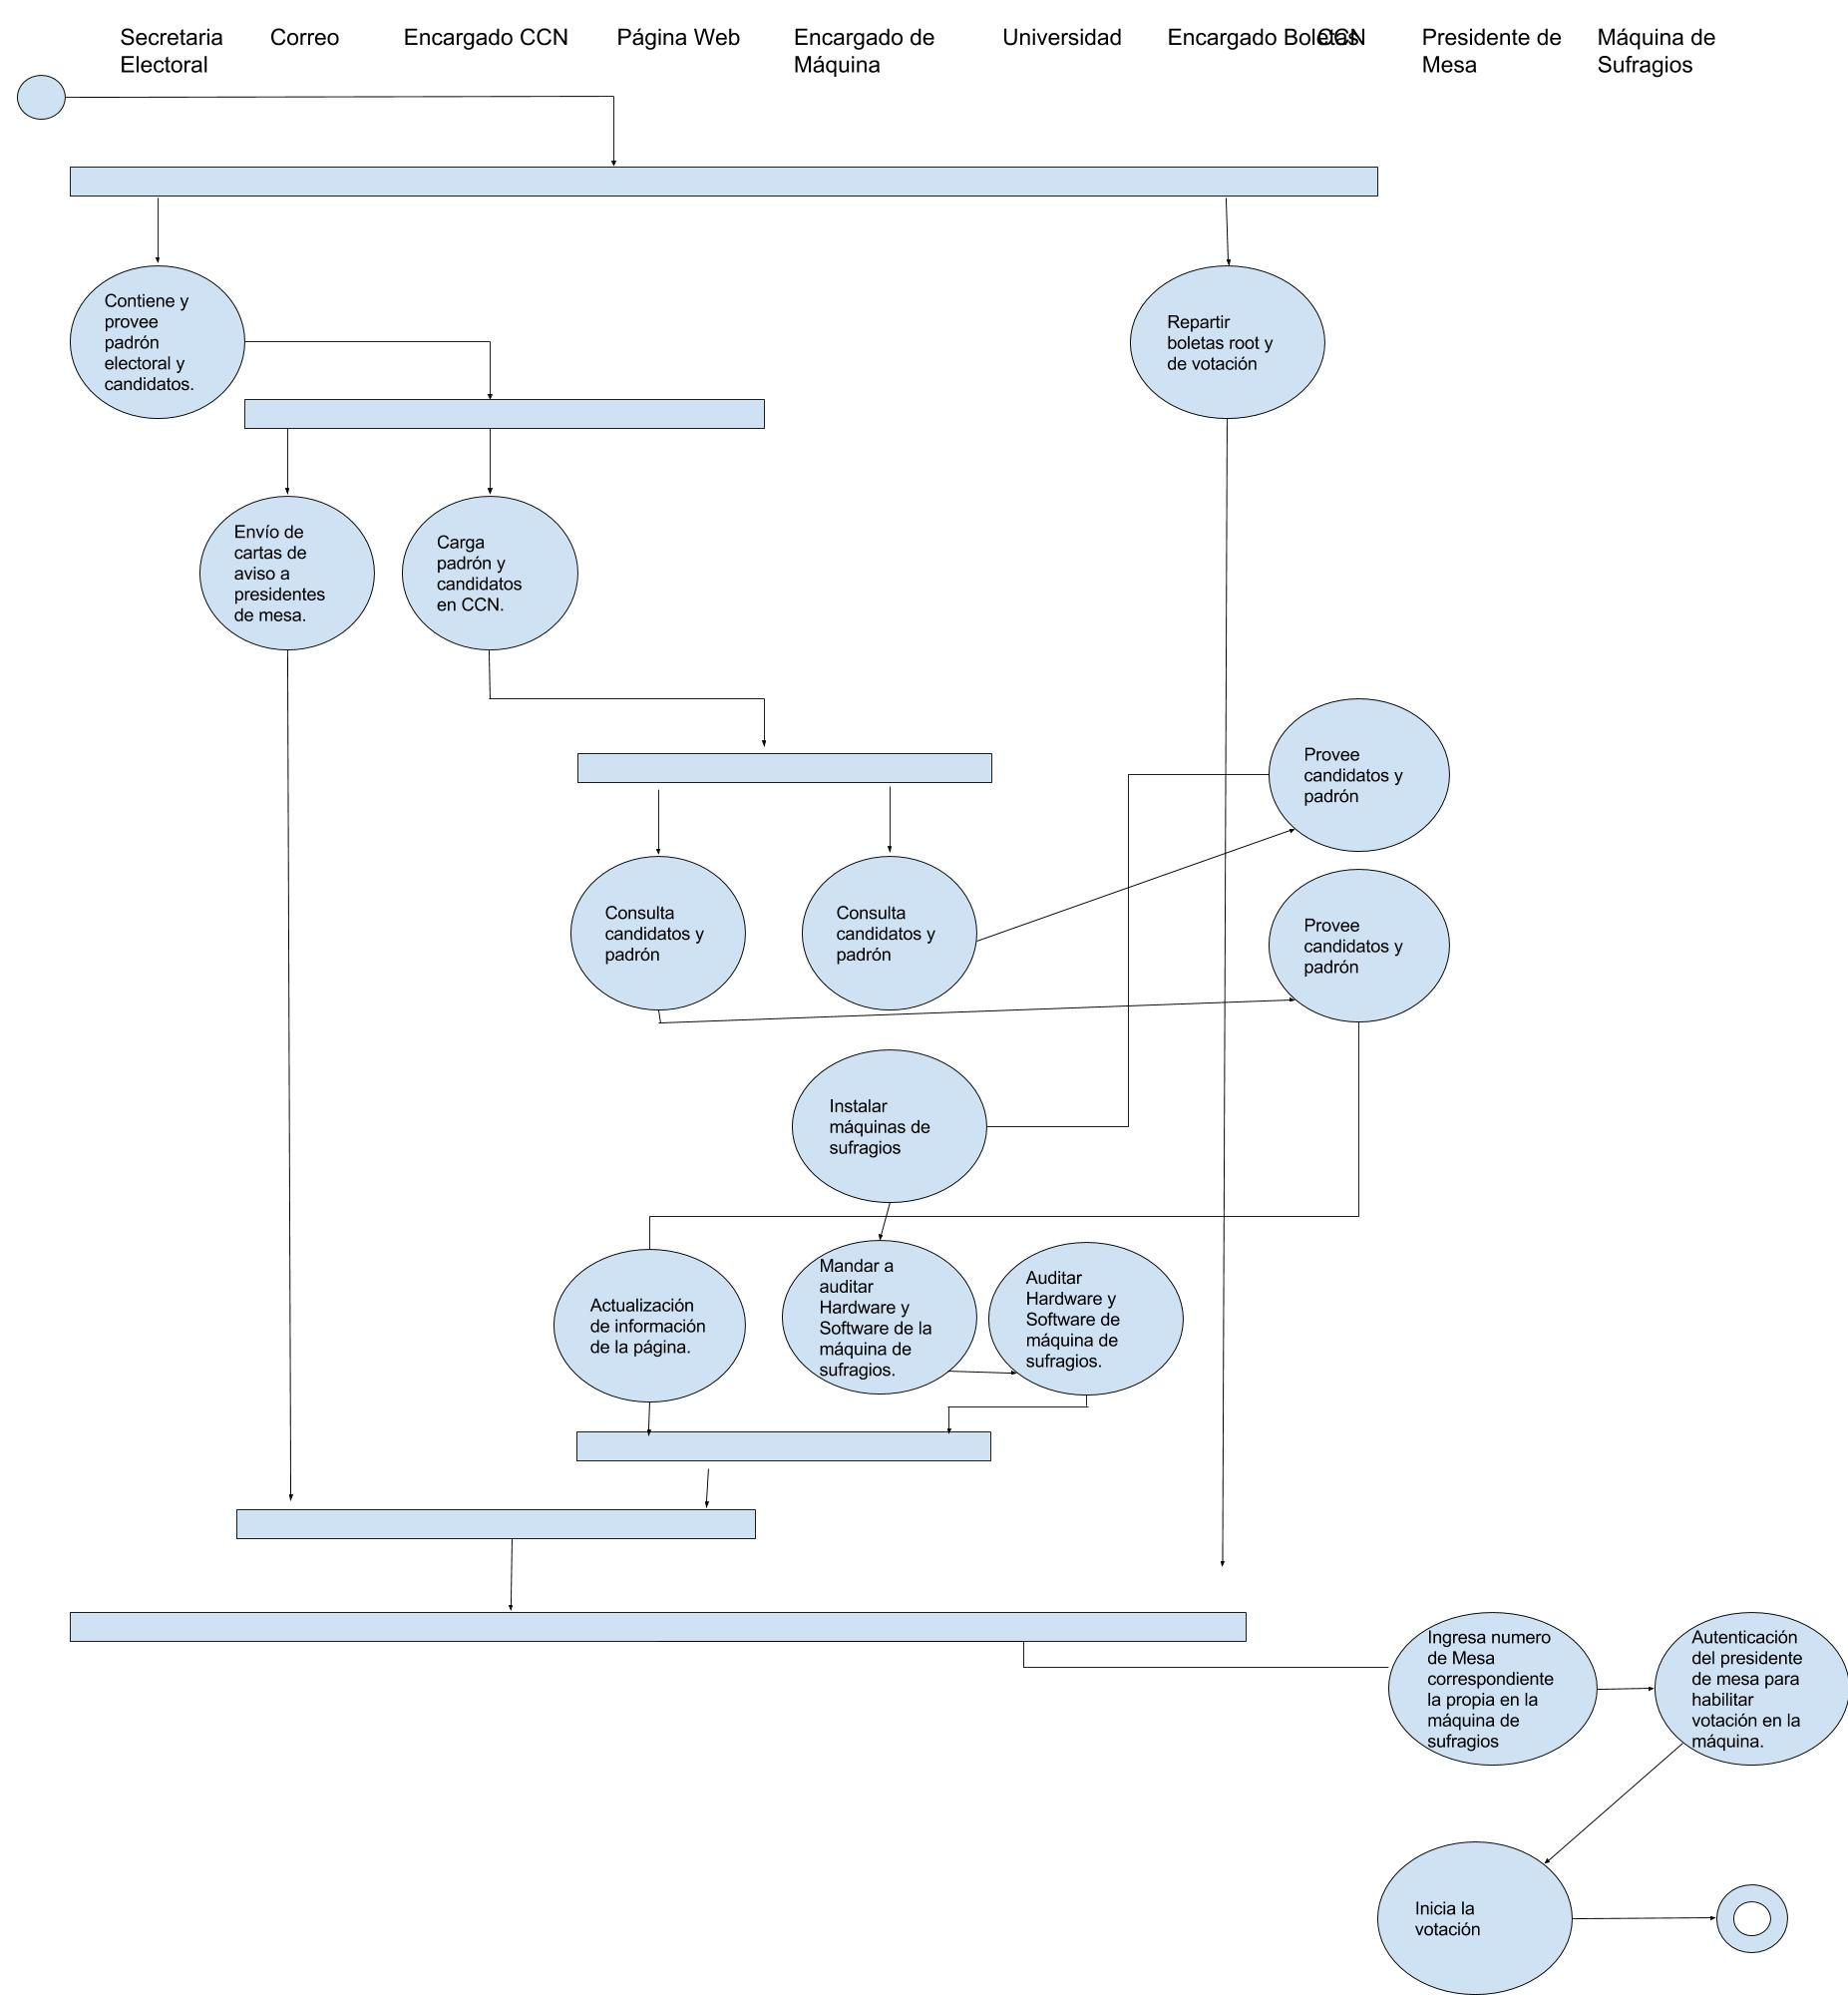
\includegraphics[scale=0.25]{imagenes/actividad/PreVotacion.jpg}
                \\
                \vspace{1pt}
                \footnotesize\textit{Diagrama de Actividad previo a la elección}
        \end{center}
\vspace{\baselineskip}


Una aclaracion pertinente de los diagramas de actividad es lo referente al abuso de notación en lo que refiere a la cardinalidad de los presidentes de mesa y de los votantes. En particular, como se podrá ver en el diagrama que habla del momento previo a la votaci\'on, donde se preparan todos los elementos que componen la infraestructura base para llevar a cabo la votaci\'on, hay descripto en actividades un \'unico inicio de la votaci\'on por parte de un un único presidente de mesa (como se vio en el caso de uso, cada presidente de mesa abre su correspondiente habilitando la m\'aquina de sufragios asociada). Por cuestiones de simplicidad, asumimos que ese flujo de actividades no corresponde únicamente a un solo presidente de mesa, sino a todos ellos.

\subsubsection{Votación}
\vspace{\baselineskip}
    \begin{center}
                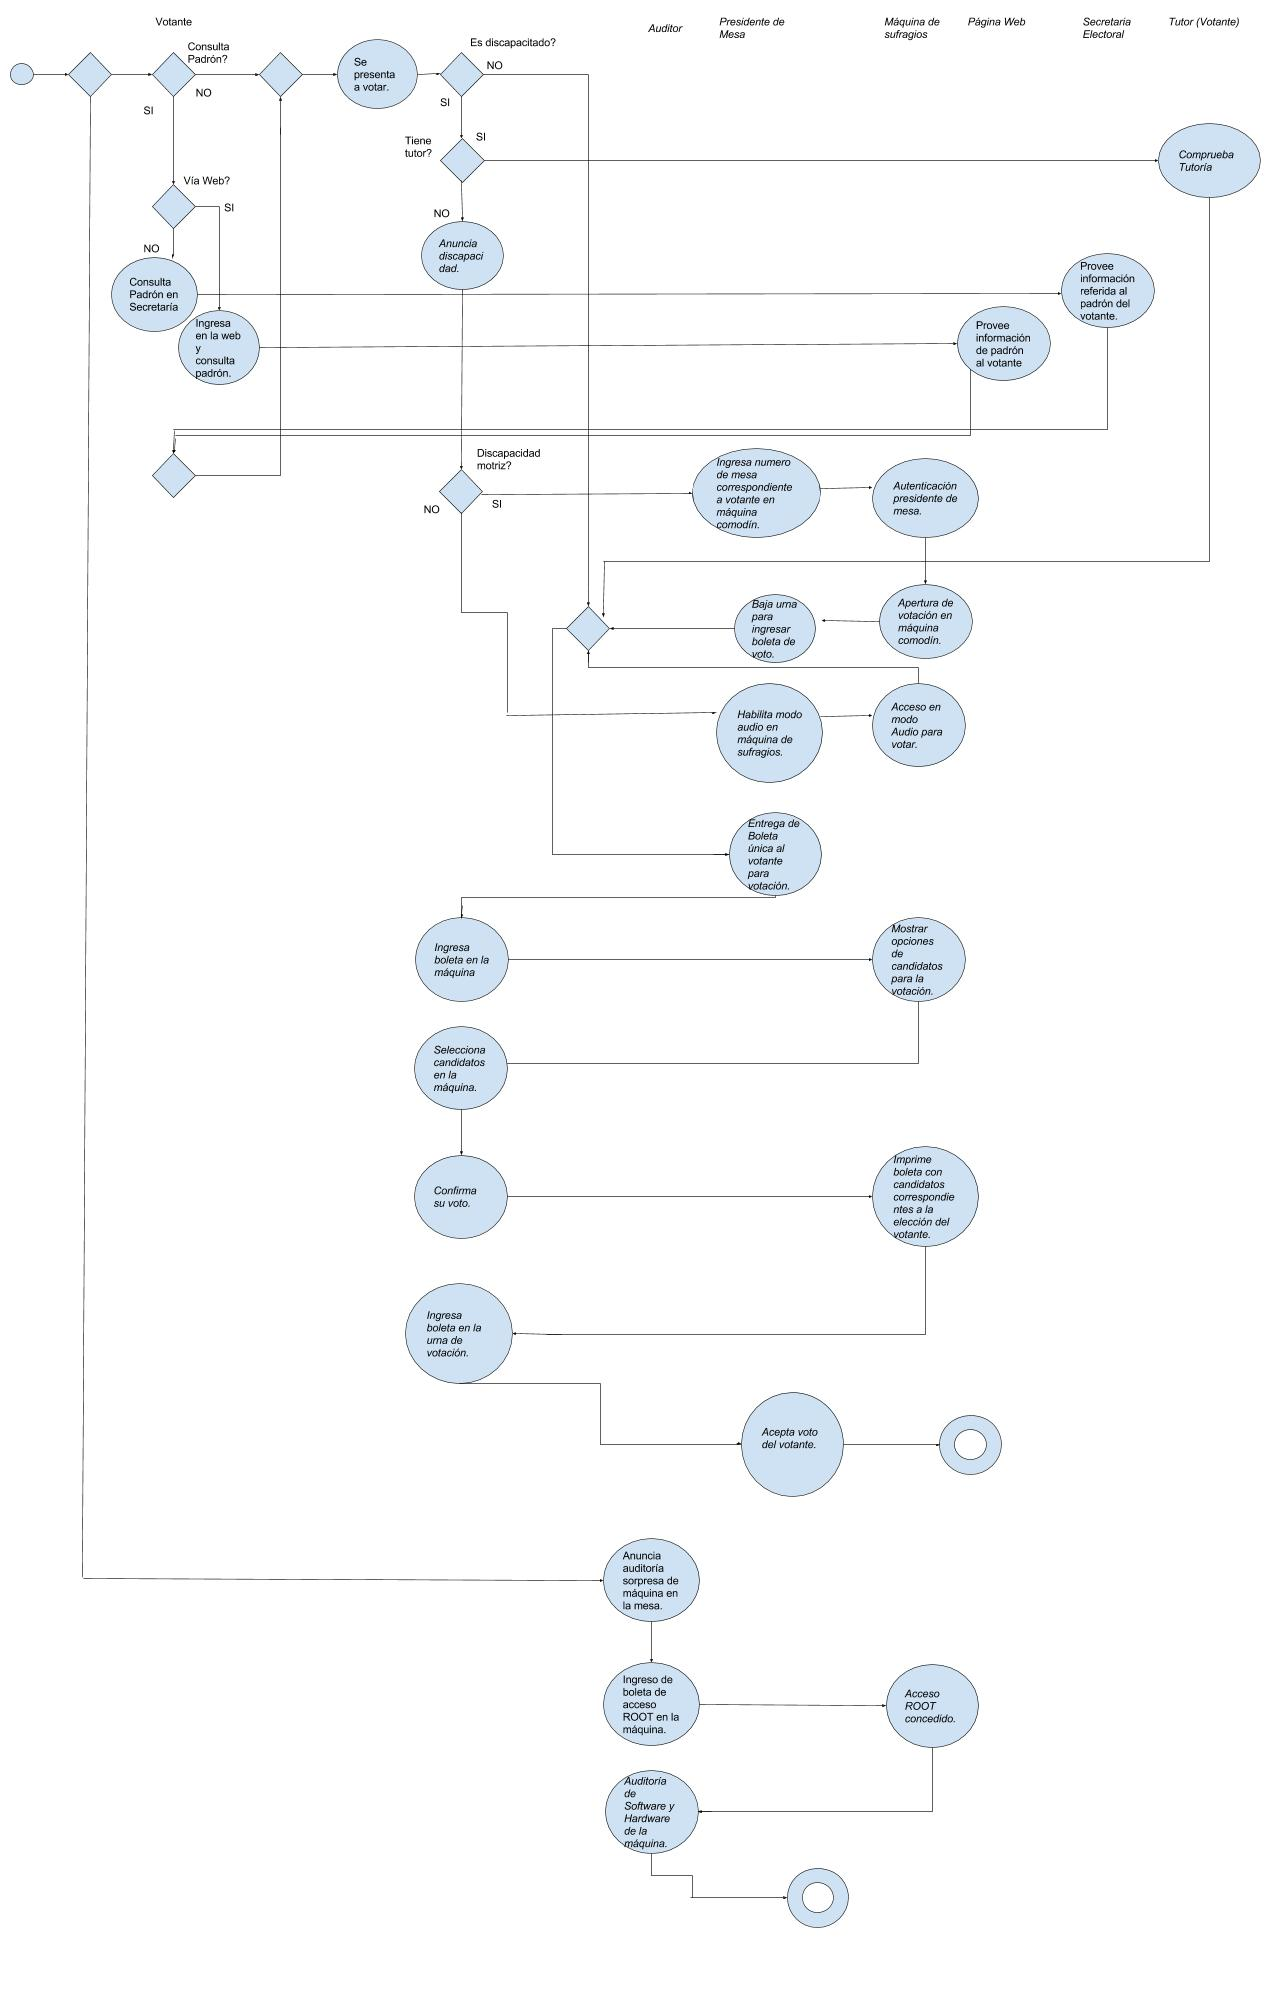
\includegraphics[scale=0.32]{imagenes/actividad/LlegadadeVotante-auditor.jpg}
                \\
                \vspace{1pt}
                \footnotesize\textit{Diagrama de Actividad durante la votación}
        \end{center}
\vspace{\baselineskip}

\par 
A su vez, ocurre lo mismo con los votantes que llegan a las diferentes mesas: para representar el flujo de un votante/auditor que viene a votar/auditar anunciandose en la m\'aquina nos limitamos a mostrar el flujo de un \'unico votante/auditor y generalizarlo para todos ellos; para simplificar el gr\'afico y porque no aporta nada intentar demostrar que la cardinalidad es superior a uno para estos conjuntos de actores en un diagrama de actividad. 
\par
Una aclaraci\'on m\'as, que habla de las actividades que son opcionales y que pueden ocurrir en cualquier momento del flujo establecido de actividades del sistema, es que dichas actividades fueron ubicadas de manera arbitraria en el diagrama en cuesti\'on pero manteniendo cierta coherencia con la l\'ogica, es decir: dichas actividades fueron situadas en momentos del diagrama donde tendr\'ia mayor sentido de que puedan llevarse a cabo que si fueran colocadas en otros sitios. (Con estas actividades nos referimos a la opcionalidad de aparici\'on, o no, de un auditor para comprobar el hardware y software de la m\'aquina de sufragios particular. Y, adem\'as, la actividad relacionada con la consulta del padr\'on que puede, o no, realizar un votante).


\subsection{FSM}
Como se mencionó previamente, nuestro sistema de voto electr\'onico cuenta con varios servidores locales. Cada uno de ellos es instalado en un colegio, para que las m\'aquinas emisoras de sufragios electr\'onicos puedan comunicarse con su servidor correspondiente. Por simplicidad, optamos por hacer el diagrama FSM de los servidores locales sobre uno solo de ellos y luego el FSM de las m\'aquinas emisoras de sufragios electr\'onicos sobre todas las m\'aquinas que corresponden a un mismo servidor. Pues para la representación general de nuestro sistema seria la repetici\'on de este escenario varias veces. Sin embargo, para el FSM de el Centro de Cómputo Nacional lo hicimos sobre la totalidad de los servidores locales para poder hacer una correcta representaci\'on.\\
En las máquinas de estado no se detalló como se realizan las auditorias y las consultas en las máquinas ya que dichos eventos los podemos ver en el gráfico de casos de usos donde se encuentran sus explicaciones sobre como se realizan mediante una boleta especial.\\
Otra aclaración más sobre este diagrama es que suponemos que puede llegar a ocurrir que una ráfaga de votos electrónicos de un servidor llegue luego de un conteo manual de otro servidor. Suponemos que puede ocurrir ya que un servidor puede demorar en enviar su última ráfaga de votos electrónicos debido a problemas técnicos o que momentaneamente se quede sin servicio de WIFI el colegio en cuestión y por otro lado existen colegios donde tienen una muy baja cantidad de habitantes por lo que provoca un rápido conteo manual de los votos. Si ambos escenarios se dan en un mismo momento entonces puede ocurrir dicho caso. Sin embargo a la vez suponemos que el arreglo de dicho conflicto se realice dentro de las 2hs para poder cumplir con el objetivo de que los resultados de las elecciones se presenten en un plazo corto de tiempo.

\par 
\subsubsection{Centro Nacional de Cómputo}
\vspace{\baselineskip}
    \begin{center}
                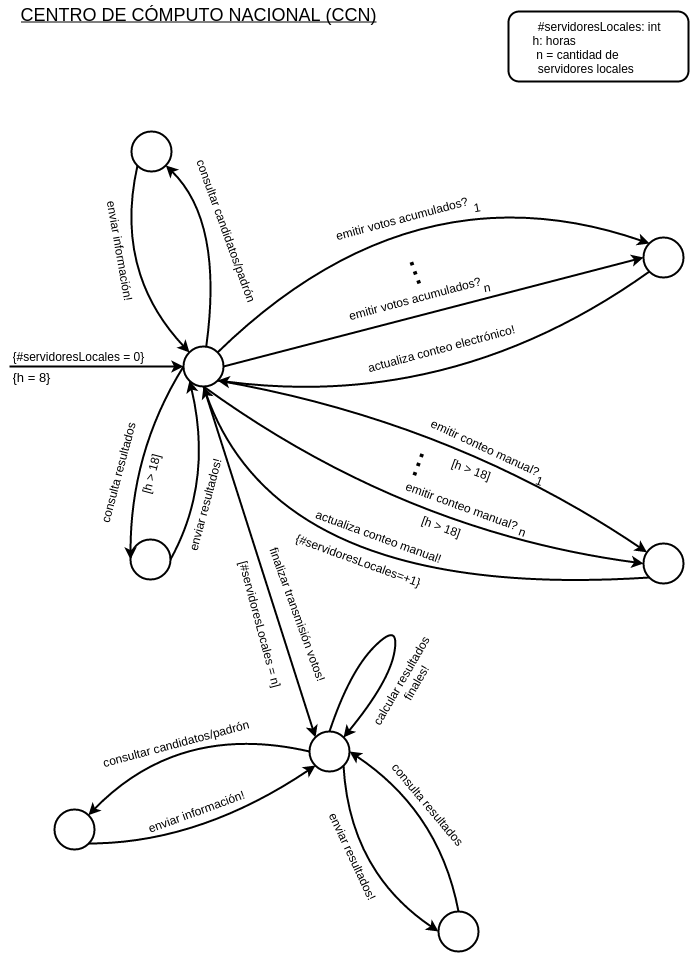
\includegraphics[scale=0.50]{imagenes/fsm/FSMCCN.png}
                \\
                \vspace{1pt}
                \footnotesize\textit{}
        \end{center}
\vspace{\baselineskip}



\subsubsection{Servidor Local}

\vspace{\baselineskip}
    \begin{center}
                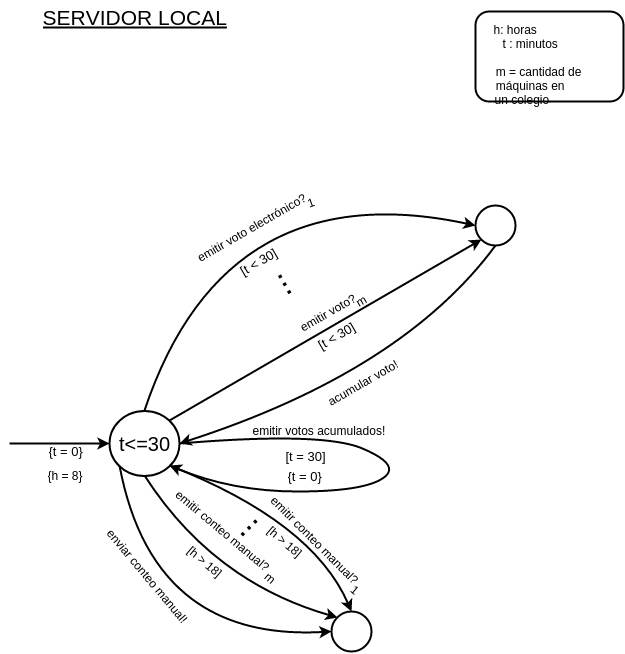
\includegraphics[scale=0.40]{imagenes/fsm/FSMservidorlocal.png}
                \\
                \vspace{1pt}
                \footnotesize\textit{}
        \end{center}
\vspace{\baselineskip}

\subsubsection{Máquina de Sufragio}

\vspace{\baselineskip}
    \begin{center}
                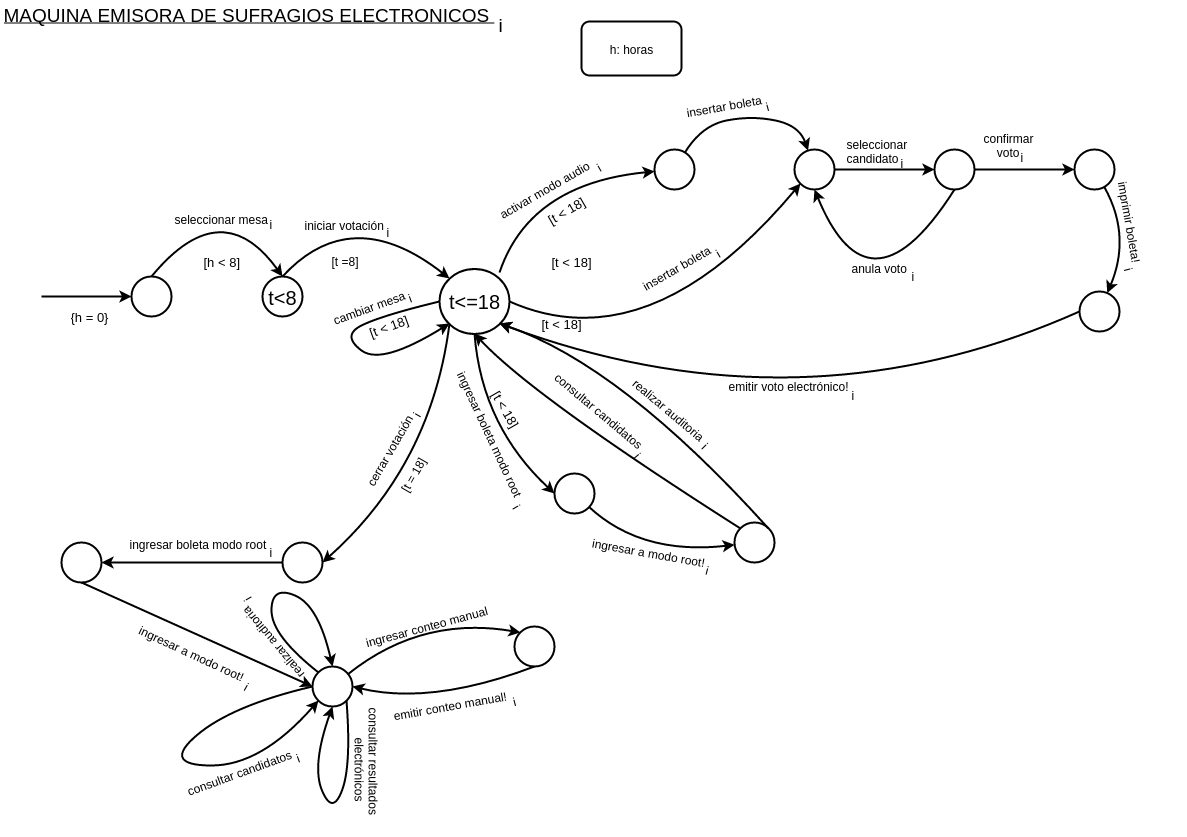
\includegraphics[scale=0.35]{imagenes/fsm/FSMmaquinaEmisoraDeSufragios.png}
                \\
                \vspace{1pt}
                \footnotesize\textit{}
        \end{center}
\vspace{\baselineskip}
En las máquinas de estado no se detalló como se realizan las auditorias y las consultas en las máquinas ya que dichos eventos los podemos ver en el gráfico de casos de usos donde se encuentran sus explicaciones sobre como se realizan mediante una boleta especial.
Otra aclaración más sobre este diagrama es que suponemos que puede llegar a ocurrir que una ráfaga de votos electrónicos de un servidor llegue luego de un conteo manual de otro servidor. Suponemos que puede ocurrir ya que un servidor puede demorar en enviar su última ráfaga de votos electrónicos debido a problemas técnicos o que momentaneamente se quede sin servicio de WIFI el colegio en cuestión y por otro lado existen colegios donde tienen una muy baja cantidad de habitantes por lo que provoca un rápido conteo manual de los votos. Si ambos escenarios se dan en un mismo momento entonces puede ocurrir dicho caso. Sin embargo a la vez suponemos que el arreglo de dicho conflicto se realice dentro de las 2hs para poder cumplir con el objetivo de que los resultados de las elecciones se presenten en un plazo corto de tiempo.
\subsubsection{Centro Nacional de Cómputo (proveedor de Página Web}
\vspace{\baselineskip}
    \begin{center}
                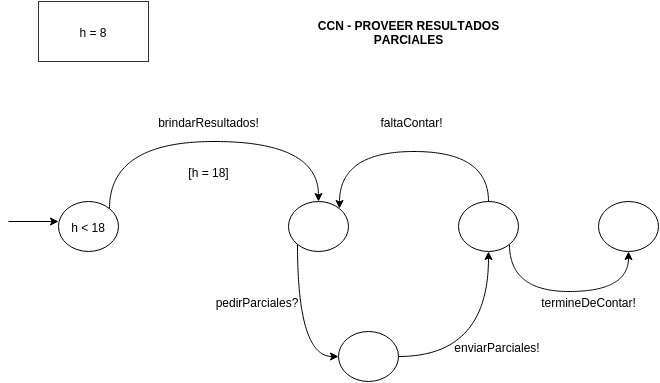
\includegraphics[scale=0.50]{imagenes/fsm/FSMCCNProveedordeWeb2.png}
                \\
                \vspace{1pt}
                \footnotesize\textit{}
        \end{center}
\vspace{\baselineskip}

\subsubsection{Página Web (Consumidor de CCN)}
\vspace{\baselineskip}
    \begin{center}
                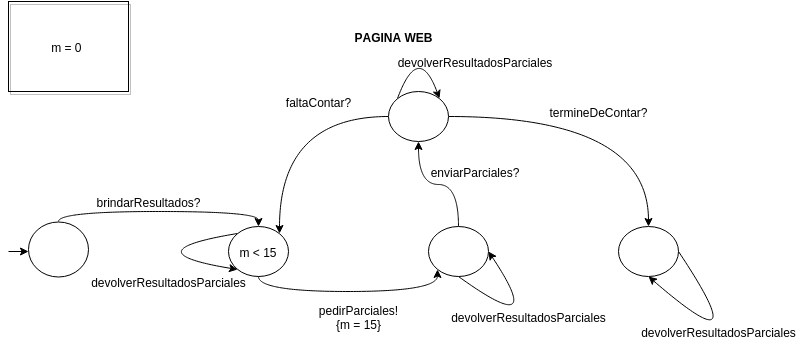
\includegraphics[scale=0.50]{imagenes/fsm/FSMWeb2.png}
                \\
                \vspace{1pt}
                \footnotesize\textit{}
        \end{center}
\vspace{\baselineskip}
\par 
\section{Discusión}

Tanto para los diagramas de actividad como para los FSM, nos encontramos el problema de la cardinalidad de elementos/actores en el sistema. En todas, tal como se mencionó, se abstrajo la idea para que sea más fácil de representar como también de comprender. Esto fue posible dado que existe un diagrama de clases que se encarga de brindar la cardinalidad faltante en los demás. De esta forma, con una conjunción de diagramas, se puede apreciar como las actividades y los estados que se modelan en realidad aplican para varios elementos en conjunto, sin necesidad de ensuciar los diagramas. 
\par
 De esta manera, ambos diagramas pudieron representar lo que realmente debían (el flujo de eventos que suceden entre actores y los cambios de estado en el diagrama de FSM).
\par 
Con el diagrama de caso de usos, decidimos enfocarnos en cómo funciona la interacción de los actores con nuestro sistema (en especial, con la máquina de sufragios, esencial para poder realizar la votación). A través del mismo pudimos revelar funcionalidad que deben poseer las partes de nuestro sistema.
\par 
El diagrama de actividad nos permitió modelar todo el funcionamiento por fuera del sistema realizado. Es decir, nos permitió explicar el proceso de votación, desde un comienzo hasta el final. Todos los eventos obtenidos a partir del diagrama de contexto pudieron ser organizados de manera tal de explicar el orden de los mismos. De esta forma, los diagramas de actividad se centraron en expresar esto.
\par 
Por otro lado, el concepto de resultados se decidió dejar de lado en el diagrama de clases debido a que el foco de esto se realizaba en los casos de uso correspondientes a las búsquedas de información a través de la página web. 
\par 
Finalmente, con el diagrama de FSM lo utilizamos para explicar la interacción entre los tres tipos de piezas de hardware que utilizamos (máquinas de sufragio, servidores locales y el Centro de Cómputo Nacional). Esto no fue especificado previamente más allá de ser conceptos importantes en nuestro diagrama de clases. Consideramos que mostrar la relación entre ambos con FSM es la decisión acertada debido a que son elementos sincronizados que envían, reciben y esperan información. Por lo tanto, tener un modelo de estados con transiciones hace muy declarativo el funcionamiento interactivo de los componentes que conforman nuestro sistema.
	
\section{Conclusión}
	Uno de los factores que consideramos interesantes y que ayudaron mucho a la hora de realizar el trabajo práctico fue la posibilidad de diferenciar partes de la especificación a partir de distintos diagramas. De esta forma, a través de la especialidad de cada diagrama se pueden mostrar distintos aspectos del problema sin perder completitud. 
\par
Utilizar un diagrama en particular para explicar cierta parte del problema permitió, por un lado, simplificar varios diagramas y dar un panorama específico y completo del problema. 
\par
 Encontramos que el diagrama de contexto resultó esencial para, a partir de él, realizar todos los gráficos. La idea general de la interacción del mundo con nuestro sistema permitió poder profundizar sobre ella sin perder la completitud que se trató de obtener en la primera instancia del trabajo práctico.
\par
 Por otro lado, como también sucedió en el primer trabajo práctico, al tratar más con el problema tuvimos que preguntarnos cosas que no lo habíamos hecho previamente, en especial para los casos de uso, donde tuvimos que plantearnos cómo funcionaría el sistema (en particular, las máquinas de sufragio).
\par
 Consideramos que las diferentes capas que atravesamos a través de los trabajos prácticos nos permitieron entender el problema desde distintos puntos de vista. A su vez, consideramos que varios de los pasos transcurridos son muy importantes a la hora de generar una especificación y de (aún más importante) entender un problema.

	%~ \newpage
	%~ \bibliographystyle{plain}
	%~ \clearpage
	%~ \bibliography{bibliography}
	%~ \addcontentsline{toc}{section}{Referencias}

\end{document}
